\chapter{Method and experiment design}\label{method}

\largerpage
The aim of the present study is to analyse and discuss the impact of integrated titles on both the audience’s perception and \isi{aesthetic experience}. While \isi{eye tracking} research and the traditional set of guidelines for subtitles have been established in audiovisual translation for quite a while now, the structure of the study and its combination of both translation studies and \isi{communication design} is innovative and unprecedented. Based on the complete analysis of the impact of the \isi{graphical translation} of text elements in film and English integrated titles that are only rarely retained in the German translation of films, a first workflow for the creation of integrated titles was drafted and tested in order to create the film material compared and discussed in this study. This chapter gives an overview of the experiment setup, the preliminary pilot study carried out in 2012, the resulting hypotheses, and the main study. As \isi{visual attention} can be measured by examining the participant’s \isi{gaze behaviour}, expressed in fixations and saccades, the \isi{eye tracker} is the most relevant part of the experiment setup and both the system and software used will be presented in the following.

\section{{Eye tracking setup}}\label{sec:7.1}

Both the pilot study and the main experiment were conducted with the Tobii TX300, a video-based \isi{eye tracking} system that uses Purkinje images.\footnote{Cf. \url{http://www.tobiipro.com/product-listing/tobii-pro-tx300/} [2016--04--12].} Its high sampling rate of 300 Hz theoretically allows for precise data and despite the high resolution of the screen (1920~x~1080~pixels), head movements did not constitute a major issue. The system collects \isi{gaze} samples, calculates and represents them as saccades and fixations, and also measures \isi{pupil size} and reports data on eyelid movements. It consists of the \isi{eye tracking} element and a removable 23’’ TFT screen, which can be used separately or in combination, as was done in the two studies. The system is accompanied by the software package \textit{Tobii Studio}. Two different versions (each up-to-date at the time of the respective study) were used in the pilot study and the main experiment and caused different challenges. Both these challenges and the overall features of the software programme are presented in \sectref{sec:7.2.3}.

\section{{Software}}\label{sec:7.2}

Besides a number of commonplace software programs such as \textit{Microsoft Excel} for the organisation of the film corpus lists and basic calculations and the \textit{R} suite\footnote{Cf. \url{https://www.r-project.org/about.html} [2016--08--08].} for “data manipulation, calculation and graphical display” (\citealt{r_project????}), three additional major tools were used in this study. \textit{Subtitle Workshop} was used in order to manage the conventional English subtitles provided by the filmmaker as well as to create the conventional German subtitles. \textit{Premiere Pro} was used to create the integrated titles, associated effects and to export the required video files. Finally, \textit{Tobii Studio} was used for data collection with the \isi{eye tracker}, AOI (area of interest) creation, and basic data analysis and export.

\subsection{Subtitle Workshop: A traditional freeware subtitling tool}\label{sec:7.2.1}

\textit{Subtitle Workshop} is freeware software created by the Uruguayan company Uruworks\footnote{Cf. \url{http://www.uruworks.net/description.html} [2016--08--09].} and is used to create subtitle files. Especially amateurs and non-profes\-sion\-als use freeware like this, while professional subtitle agencies generally use their own software or a commercial product. \textit{Subtitle Workshop} consists of several modules that can be activated individually. These include a preview window and the subtitle window. Additionally, a second subtitle window can be activated for translation, making it possible to see both source and target subtitle at the same time. The in and out times can be selected either through the preview window or manually. The subtitle files can then be saved in a wide range of file formats, such as the popular subrip format (.srt)\footnote{Explanations of various subtitle formats can be found here: \url{http://www.afterdawn.com/guides/archive/subtitle\_formats\_explained.cfm} [2016--04--18].} that is highly compatible and allows integration into videos, DVDs, BDs or upload to YouTube. While \textit{Subtitle Workshop} is suitable for creating basic subtitle files and therefore sufficient for creating the conventional subtitle files used in the studies, other freeware software such as \textit{Aegisub} allows for a wider range of data formats and additional features such as individual \isi{placement} in the image. No issues arose during work with \textit{Subtitle Workshop} and the handling was easy and productive.

However, while software such as \textit{Aegisub} allows individual positions of titles and a range of colour and format features, sophisticated effects can still best be achieved with professional video editing software. Therefore, \textit{Adobe Premiere Pro} was used to create the integrated titles for both the pilot and the main study.

\subsection{Adobe Premiere Pro}\label{sec:7.2.2}

\textit{Adobe Premiere Pro} is a commercial video editing and cutting software from the American software company Adobe Systems. For the pilot study, the then up-to-date version CS6, released in May 2012, was used. The main study made use of the latest versions \textit{Premiere Pro} CC and \textit{Premiere Pro} CC 2015. As \textit{Premiere Pro} is part of Adobe’s ‘Creative Suite’, it shares many features with other products of the suite (such as \textit{Photoshop} and \textit{After Effects}) and therefore allows for an easier data exchange between these programs – e.g. graphic elements created in \textit{Photoshop} can be imported into \textit{Premiere Pro}.

\textit{Premiere Pro} offers various tools for cutting and editing video material. For the pilot study, scenes had to be cut out of the film material used and combined into one file. For both the pilot study and main experiments, the integrated titles were created using the title tool in \textit{Premiere Pro}. It makes it possible to place titles within the whole image and use effects on them such as masks (if parts of the title should be ‘covered’), kinetic motion effects, or 3D effects. After creating the titles, they can be added to the video’s timeline and the exact point in time they are to be displayed can be chosen. The project can then be exported and saved in most common video formats.

\subsection{Tobii Studio}\label{sec:7.2.3}

For the present study, the software offered by the manufacturer of the \isi{eye tracker}, \textit{Tobii Studio}, was used. It makes it possible to design and execute the experiment and then offers various tools for both data visualisation and analysis. As visualisation “gives a very good first impression” (\citealt{Hvelplund2014}:~215), most \isi{eye tracking} systems offer some kind of software that does visualisation (\citealt{Hvelplund2014}:~212). \textit{Tobii Studio} can display the current \isi{fixation point} in a video of the materials looked at by participants, add a static \isi{scan path} with numbered fixations to a still image of the material, indicate \isi{fixation duration} visually, indicate individual participants, and present saccades as lines between \isi{fixation} points. As visible from \figref{fig:FIG48fig46}, the eye movement data of one or more participants can be visualised in heat maps, \isi{gaze} plots, or bee swarms (several animated \isi{fixation} points indicate the various participants at the same time).

\begin{figure}
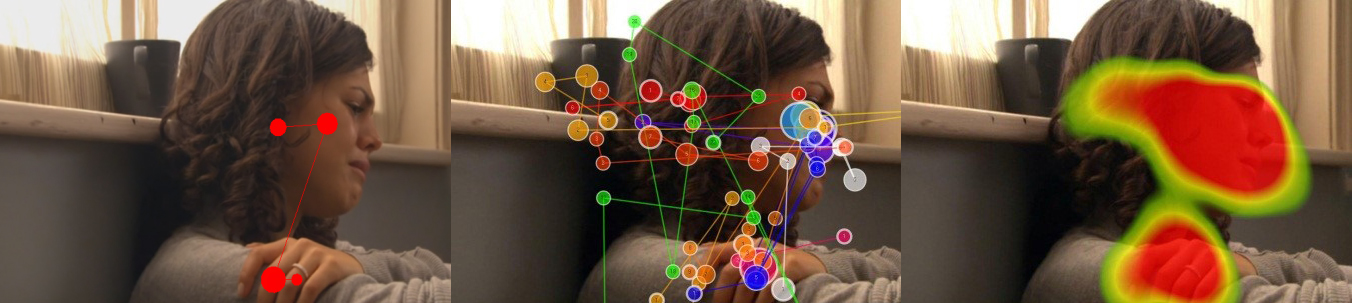
\includegraphics[width=\textwidth]{figures/FIG48fig46.jpg}
\caption{Visualisation of eye tracking data by \textit{Tobii Studio} (scan path, accumulated scan path, heat map; \textit{Being Human} S01E01, UK 2008--2013)}
\label{fig:FIG48fig46}
\end{figure}

While it was used extensively during the pilot study, it mostly just provided an overview during the main experiment. However, the automatic cluster recognition tool was used to identify relevant focus areas in the image and compare \isi{visual attention distribution} between the different modes. \isi{AOIs} were used statistically to calculate \isi{fixation duration} on the subtitle or \isi{title area} and the overall image as well as reaction times (see \sectref{sec:8.1}). The \isi{AOIs} in the studies were created by hand and can be given shapes such as squares or circles but also freely drawn shapes. Issues mainly occurred during the pilot study and will be discussed in the following chapter.

\section{Pilot study}\label{sec:7.3}

The pilot study for this experiment was conducted in June and July 2012 at FTSK Germersheim, Johannes Gutenberg University Mainz.\footnote{In the course of the Master’s thesis “Integrated Titles – An Alternative to Traditional Subtitles” \citep{Fox2012}.} While it included a substantial number of participants, only little statistical data could be retrieved due to faulty raw data and significant limitations of the software used. The aim was to not only test the equipment and software but also the process of creating integrated titles – at this point without any specific set of rules besides the goal of placing titles in a way that would allow easier \isi{speaker identification} and provide an indication of the \isi{speaking direction} – and verify the basic validity of the first set of general hypotheses:

\begin{itemize}
\item Compared to viewers of conventional titles, the viewers of integrated titles will be able to spend more time exploring the image instead of reading the title.
\item The saccades of the viewers of integrated titles will be shorter compared to the saccades of viewers of conventional titles.
\item The overall \isi{gaze behaviour} of viewers of integrated titles will be closer to that of English natives who are not distracted by titles.
\item The viewers of integrated titles will report a better \isi{aesthetic experience}.
\end{itemize}

The equipment included the identical \isi{eye tracker} Tobii TX300 and the then latest version of \textit{Tobii Studio}. Additionally, the questionnaire on the \isi{aesthetic experience} and subjective \isi{information intake} for this study was to be tested.

The participants for the pilot study came from the student body – both undergraduate and graduate students – and staff of FTSK. A total of 52 participants volunteered for the pilot study, 16 of them were English native speakers and 36 were German native speakers. The German native speakers stated that – in their subjective opinion and habit – they needed German subtitles to watch English film material. As the use of subtitles is a personal and subjective decision, the English language proficiency was not tested.

The pilot study used the first episode of the first season of \textit{Being Human} as source material. BBC describes \textit{Being Human} as a “supernatural drama” and “dramedy”,\footnote{Cf. \url{http://www.bbc.co.uk/programmes/b00hqlc4} [2016--04--05]} referring to its mixture of fantasy, horror, drama and comedy. The first episode was broadcast in December 2008 on \textit{BBC Three}. \textit{Being Human} tells the story of Annie, George and Mitchell, who strive for a normal ‘life’. Over 100 years old, Mitchell is the oldest of the unlikely group of friends and a vampire who renounced drinking blood 50 years ago, but still fights his thirst for blood every day. George was bitten by a werewolf and has had to fight his own inner monster ever since. Mitchell and George meet and decide to fight their demons together. Soon, they rent a little house and meet the former resident Annie, a ghost who is not done with life. Together, they want to become part of human society again. In doing so, everyone encounters his or her own very personal limits. Even though the total of five season was very successful in the UK, it never reached the German market – neither dubbed nor with subtitles. However, the American remake, produced by the BBC America, was broadcast on the German private channel \textit{ProSieben}.\footnote{Cf. \url{http://www.serienjunkies.de/news/prosiebensat1-sichert-usversion-being-human-33444.html} [2016--04--05].}

The study was split into three steps: In the first step, the 16 English natives watched the whole episode in its original version (OV; without any subtitles or other edits), while the eye movements were recorded. One recording had to be excluded due to a loss of signal, wherefore only 15 recordings could be used in the analysis. The \isi{gaze} plots and heat maps for each scene containing spoken content showed the \isi{main focus} points or areas in these scenes that were later used as a basis for the comparison with the traditional subtitles (TS) and the integrated titles (IT).

The second step included the creation of the German subtitles\footnote{In cooperation with Matthias Balzer. Permission for use of the episode was given by both the BBC and the production studio Touchpaper.} and the \isi{eye tracking} recordings with 15 German native speakers. They watched the episode in the TS condition and all recordings could be used in the analysis. The participants watched the whole episode with the German subtitles. These recordings were then analysed and compared to the recordings of the OV condition. Due to problems arising with the amount of data and clean \isi{scene selection}, the decision was made to classify all suitable scenes according to their level of complexity (cf. \citealt{Fox2012}). Four levels were defined and one scene per level was chosen as well as one additional scene of the lowest level as these scenes of lower complexity account for most of the analysed episode. The duration per scene was about 1 to 2 minutes. In the third step, the integrated titles were created, based on the \isi{main focus} points and areas identified in the analysis of the OV recordings. Further \isi{placement} strategies were the following:

\begin{itemize}
\item Place titles close to focus of the native participant group
\item Indicate speaker
\item Indicate \isi{speaking direction}
\item Produce \isi{sufficient contrast}
\item Do no cover relevant image areas or elements
\end{itemize}

A total of 21 German natives watched the IT condition while their eye movements were recorded. Of these recordings, 15 were suitable for analysis. After that, the participants were asked to fill in a questionnaire and 17 of the participants agreed. The following statements had to be rated in the questionnaire:

\begin{enumerate}
\item I could easily read all titles.
\item I received all necessary information through the titles.
\item I would like to watch a whole film with integrated titles.
\item I would prefer integrated titles over traditional subtitles.
\item If you prefer \isi{dubbing} over subtitles (if not, please continue to question 6): I would prefer integrated titles over \isi{dubbing}.
\item I had more time to explore the image with integrated titles (compared to traditional subtitles).
\item The integrated titles did not cover any relevant areas or elements in the image.
\item The integrated titles did not distract me from the image.
\item Due to the integrated titles, I perceived more details in the image.
\item Please rate your \isi{overall aesthetic experience} with the integrated titles (1: very good; 4: very bad).
\end{enumerate}

The participants had to rate the statements on their comprehension, \isi{usability} of the titles, and \isi{enjoyment}, using a Likert scale with the option 1 (completely agree) to 4 (completely disagree). The questionnaire was the only part of the pilot study that was sufficient for statistical analysis (see \figref{fig:FIG49chart3}).

\begin{figure} 
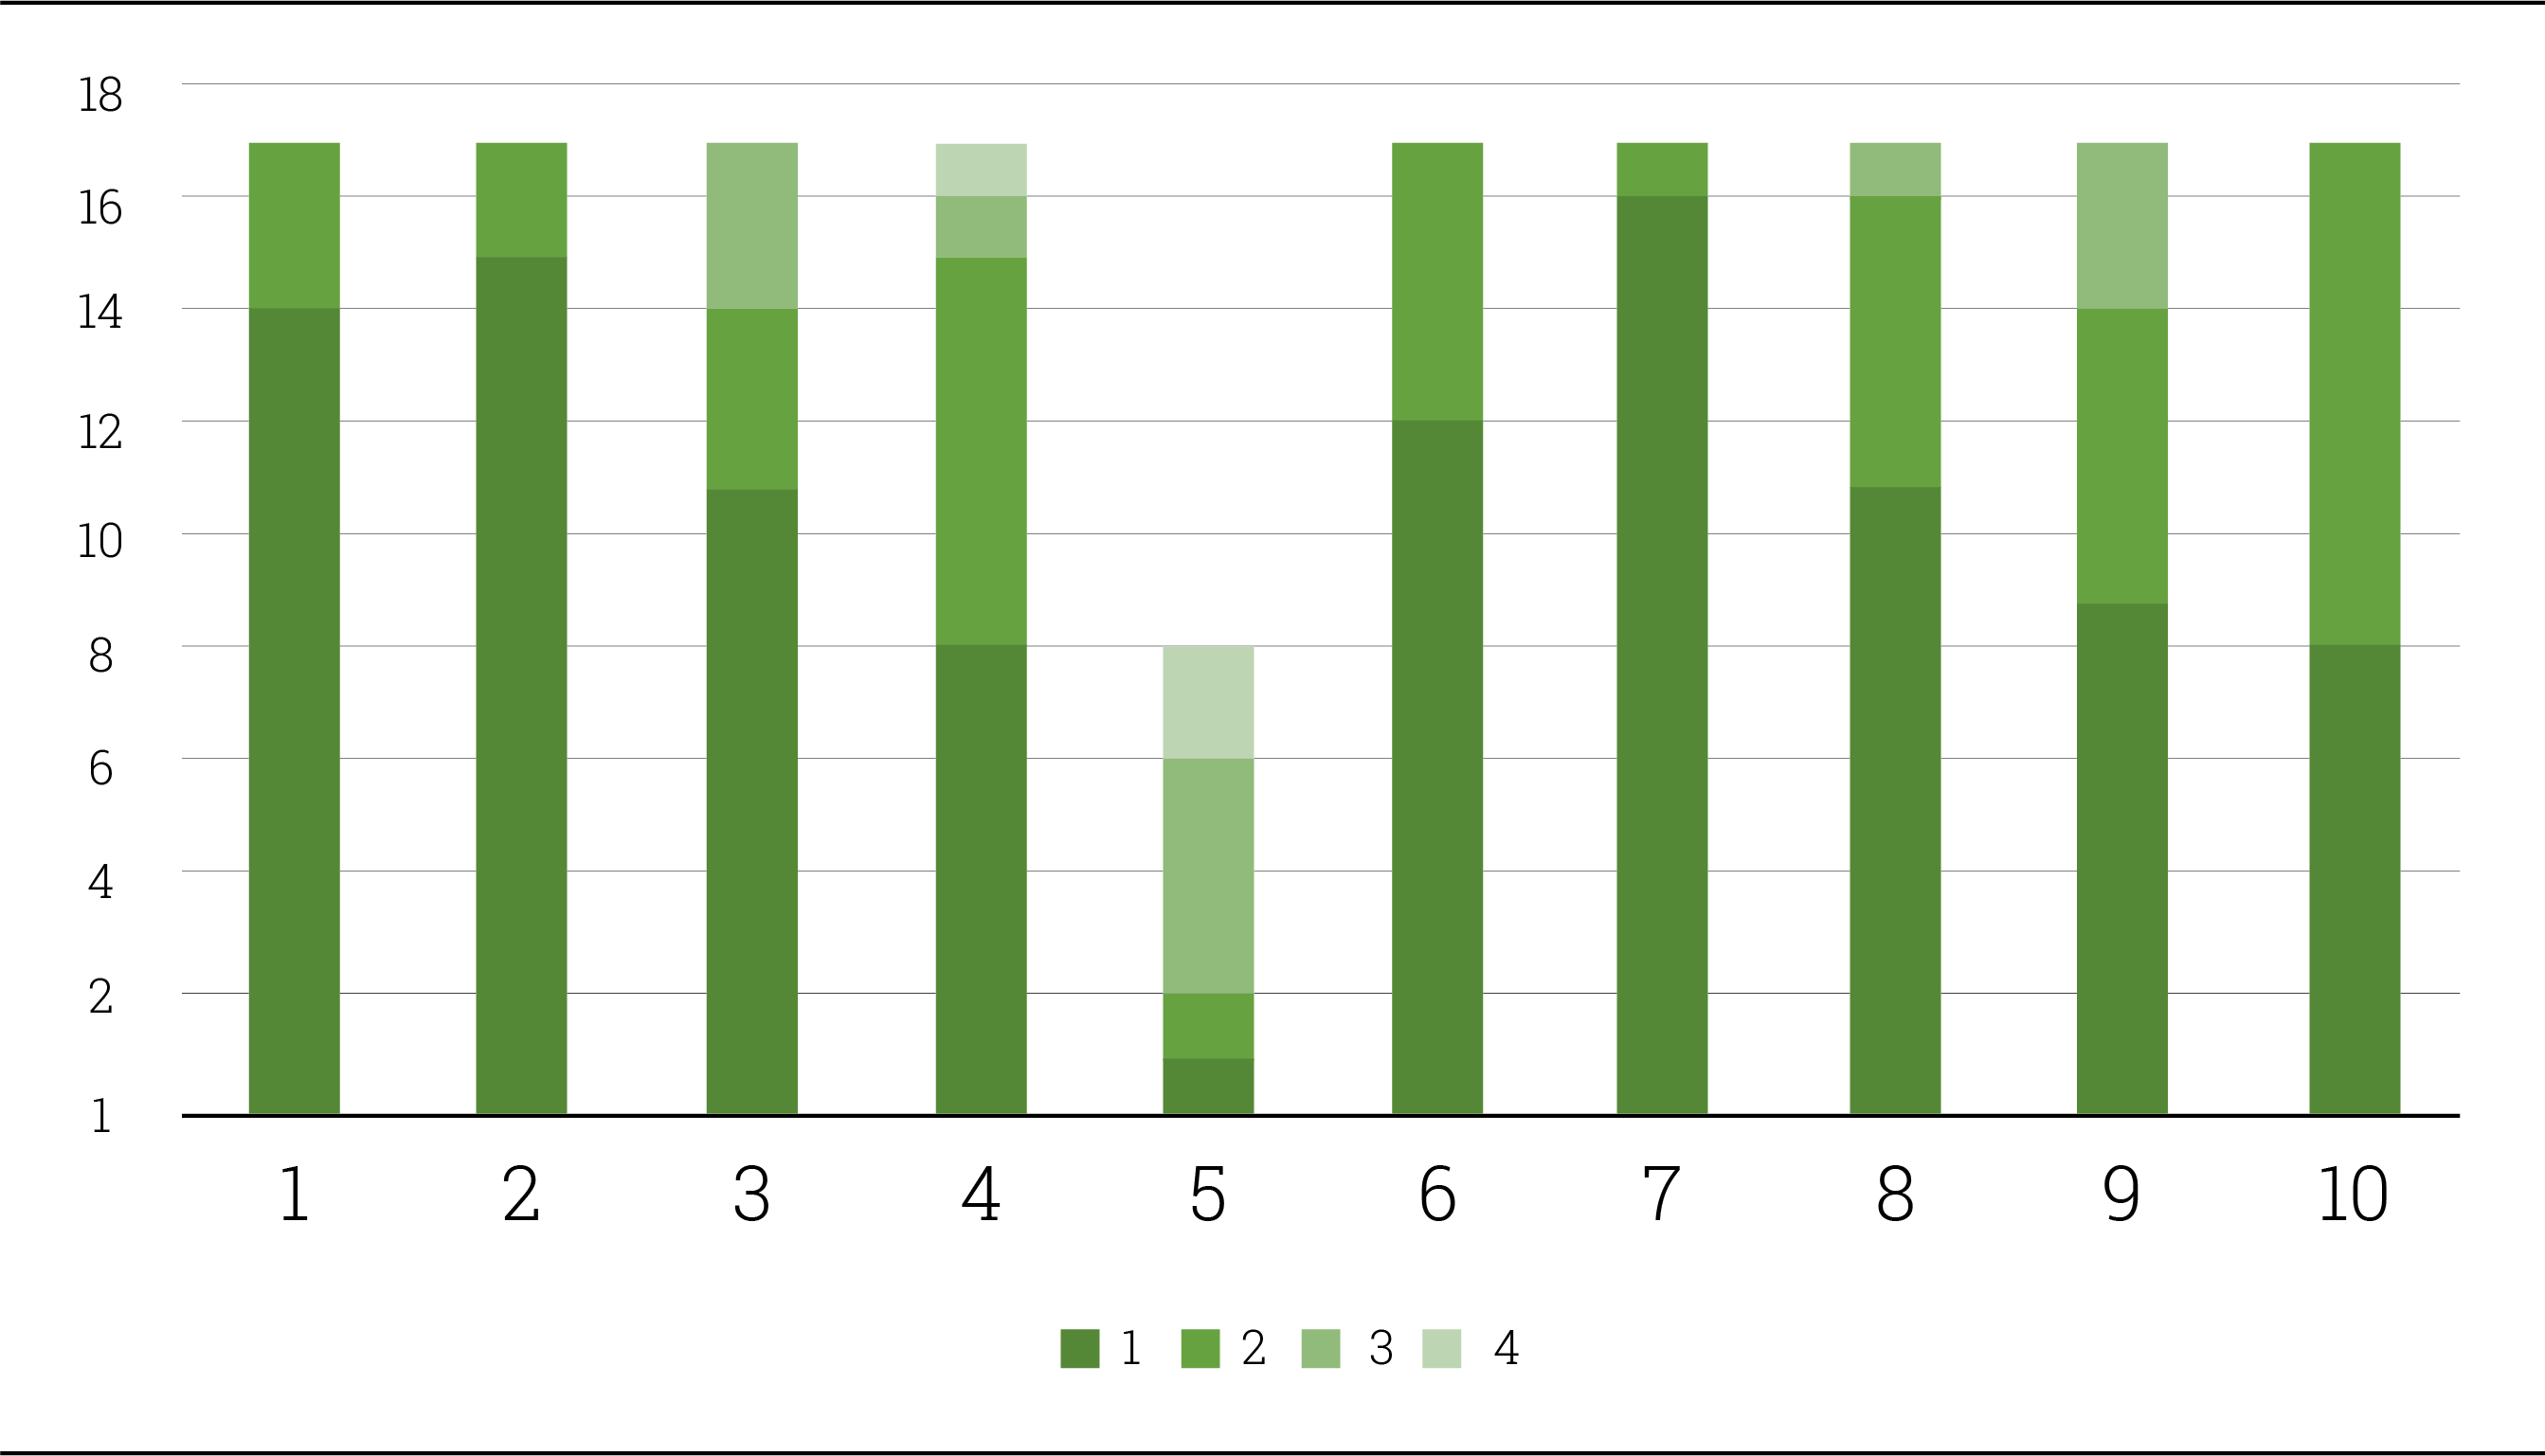
\includegraphics[width=\textwidth]{figures/FIG49chart3.png}
\caption{Questionnaire evaluation with the scores of 1 (completely agree) to 4 (completely disagree).}
\label{fig:FIG49chart3}
\end{figure}

The pilot study showed that scenes of the lowest level of complexity create little difference between conventional subtitles and integrated titles concerning the \isi{split attention}\footnote{Chandler and Sweller define “\isi{split attention}” as the result of the divided attention of a learner due to “multiple sources of information” (\citeyear{Chandler1991}:~295), which can be – in the context of film material – transferred to splitting attention between image and title (and sound) as sources of information. More attention towards the image – rather than on the subtitle or title – was considered a positive effect as easier and faster information processing is more likely.} and main \isi{attention distribution}. However, the more movement and content complexity increase, the more the participants of conventional subtitles focused on the \isi{subtitle area} and only infrequently paid attention to the actual image. This became visible from the analysis of the \isi{gaze} plots and heat maps. The integrated titles, on the other hand, and regardless of scene complexity, created a balanced focus with participants sometimes even paying more attention to the image than the titles. The questionnaire evaluation showed that the majority of the IT participants rated their \isi{aesthetic experience} and information gain as good, also in comparison with conventional subtitles. This strengthens the hypothesis that \isi{aesthetics} play an active part in how film is perceived and processed.

Several issues were encountered during the pilot study. One of the main issues was the large amount of data produced by the first two sets of recordings. These recordings were about 50~minutes each. Due to incomprehensible issues in \textit{Tobii Studio}, scenes smaller than 10~seconds could not be selected in a clean way. Start and end times often changed after selection, even if done by hand. Therefore, none of the features of \textit{Tobii Studio} that offer automatic processing and creation of data could be used. Due to this software error, these often too long and temporally displaced scenes – of which there were several hundred – had to be corrected later by hand. This allowed basic analysis of the then produced heat maps and \isi{gaze} plots but did not leave the time to create any statistical data on e.g. first fixations or \isi{fixation} durations.

Besides these issues, the pilot study proved to be a good test of the first basic set of hypotheses. Furthermore, a first concept for the analysis of \isi{image composition} and \isi{typographic identity} emerged, and a first set of \isi{placement} strategies (based on the accumulated \isi{eye tracking} data) and effects could be tested. The following chapter will present the refined hypotheses that were then tested in the main study.

\largerpage[-1]
\section{Hypotheses}\label{sec:7.4}

Based on the pilot study, it was assumed that integrated titles, compared to traditional subtitles, would have an effect on the \isi{fixation duration}, the time to \isi{first fixation} in the \isi{title area}, the \isi{attention distribution} between image and title, the \isi{aesthetic experience} of the audience, and the \isi{information intake}. The following aspects of \isi{visual attention} and the \isi{viewing experience} of film audiences are relevant for the main study:


\begin{itemize}
\item \textit{Fixation duration in the title area}: The \isi{fixation duration} is measured from the first to the last \isi{fixation} on a subtitle or title. The data evaluation in the pilot study indicated a decreased \isi{fixation duration} compared to traditional subtitles. The participants seemed to re-read integrated titles less often and were more motivated to quickly return to the focal points in the image.
\item \textit{Saccade length}: The length (or duration) of a \isi{saccade} describes the distance (or time) between one \isi{fixation point} and the next. As no information is absorbed during saccadic movements, it seems likely that shorter saccades allow for a higher \isi{information intake} and long saccades for a lower intake. Due to the \isi{placement} closer to the focal points, integrated titles might induce shorter saccades.\footnote{While this measure showed promise, the raw data concerning the saccades turned out to be unreliable and faulty, especially concerning the definition and length of saccades. It seems like proper scripts or finer software are required to analyse this type of data. It was therefore not analysed in this study.}
\item \textit{Correspondence to natural focus}: To allow for a \isi{viewing experience} that is as close to that of a native viewer that watches the film without any titles, the \isi{gaze behaviour} should be as similar as possible and the same \isi{main focus} points should be fixated.
\item \textit{Reaction time}: This term describes the duration from when the subtitle or title fades in until the \isi{first fixation} by the viewer. If this time is increased considerably by integrated titles, this could be a counterargument for individual \isi{placement}. As this seems to be the main concern of critics of integrated titles, the reaction times of traditional subtitles and integrated titles should be compared and their difference discussed.
\item \textit{Aesthetic experience}: The participants for the integrated titles will be asked to fill in a questionnaire on their \isi{aesthetic experience} and rate it compared to traditional subtitles.
\end{itemize}

\newpage 
Based on these initially defined aspects, the following hypotheses on integrated titles (IT) and traditional titles (TS) emerged:

\bigskip
Visual attention (based on \isi{eye tracking}):

\begin{itemize}
\item Hypothesis 1:   Fixation duration in the \isi{title area} is shorter for IT than for TS.
\item Hypothesis 2:   IT participants spend more time fixating (exploring) the image than fixating (reading) the titles, experiencing a \isi{positive split attention}.
\item Hypothesis 3:   The focus of the IT participants resembles the \isi{natural focus} of the native viewers considerably more than the focus of the TS participants.
\item Hypothesis 4:  The \isi{reaction time} of the IT participants is higher than that of the TS participants.
\end{itemize}

\bigskip
Aesthetic experience (based on questionnaire):

\begin{itemize}
\item Hypothesis 5:   The IT participants experience a higher \isi{information intake}.
\item Hypothesis 6:   The integrated titles are rated as more \isi{aesthetic}.
\end{itemize}

In this study, these hypotheses are tested and discussed based on the collected \isi{eye tracking} and questionnaire data. Each recording session started with the participant being introduced to the \isi{eye tracking} lab and the \isi{eye tracker}. The participant would then watch the episode without any prior knowledge of the topic or the goal of the experiment. The German native speakers who watched the version with the integrated titles would then fill in a questionnaire designed to cover subjective information flow and \isi{aesthetics} of the titles.


\section{Main study}\label{sec:7.5}

Based on the insights gained from the pilot study, the main study tested the developed hypotheses. Based on the skill and rule sets developed in \chapref{integrated}, \chapref{placement}, and \chapref{workflow}, as well as the \isi{eye tracking} studies discussed in \sectref{sec:6.3.2}, the main study consisted of the following steps:

\begin{enumerate}
\item Analysis of the \isi{image composition}, \isi{typography}, and content of the used film material – includes interview-based data with filmmaker Pablo Ro\-me\-ro-Fresco and \isi{eye tracking} data of participants watching the original film.
\item Translation of the English original subtitles into German.
\item Creation of two sets of titles: Conventional German subtitles following the guidelines and strategies described in \sectref{sec:1.2}, and German integrated titles based on the adjusted guidelines described in \sectref{sec:7.5.3.1}.
\item Title design and \isi{placement} based on the \isi{typographic identity} of the film (see \sectref{sec:2.3}) and the rules summaries in \sectref{sec:3.5} and \sectref{sec:4.3}.
\item Data recording through \isi{eye tracking} of the film with either conventional subtitles or integrated titles and a \isi{post-hoc questionnaire}.
\item Data evaluation and discussion.
\end{enumerate}

The following chapters will give on overview over the participants of the study, the film material, and the adjustments made to the conventional subtitling guidelines.

\subsection{{Participants}}\label{sec:7.5.1}

All in all, 45~volunteers participated in the experiment. Of these participants, 14 were native speakers of English between the age of 18 and 45 who study at the FTSK Germersheim, Johannes Gutenberg University Mainz, Germany, and watched the original version of the short documentary \textit{Joining the Dots}. As film audiences are usually not homogeneous groups, no other characteristics besides native language and eye sight were determined. Each participant claimed to have normal or corrected-to-normal vision. Thirty-one participants were German native speakers who stated that they rely on German subtitles to understand English films. As using subtitles is a personal decision based on the viewer’s self-assessment and not his or her factual knowledge of the foreign language, the actual level of the participants’ English was not determined. Of these participants with German as their native language, 15 watched \textit{Joining the Dots} with traditional subtitles in German. The other 16 German participants watched the film with the integrated titles. None of the participants had seen the documentary before.

\subsection{{Material}}\label{sec:7.5.2} 
\textit{Joining the Dots} is a short documentary by Pablo Romero-Fresco, screened for the first time in 2012.\footnote{For further information on \textit{Joining the Dots}, see \url{http://www.jostrans.org/issue20/int\_romero.php} [2014--10--28].} The documentary shows an interview with Trevor Franklin who went blind at the age of 60. He speaks about his experiences and how he handles the disability. The main topic of the documentary is accessibility for the blind, focusing on television and theatre. In an interview with Pablo Romero-Fresco, the \isi{image system}, compositions and key elements in the various scenes were defined and possible placements and designs discussed. Due to its documental character, \textit{Joining the Dots} offers a simple \isi{image system}\footnote{For a definition of “\isi{image system}” see Mercado (\citeyear{mercado2010}:~21): “[…] refers to the use of recurrent images and compositions in a film to add layers of meaning to a narrative. … Because the experience of watching a film relies so much on the use of images ([…]), most films have an \isi{image system} at work at some level, whether the filmmaker intends to have one or not.” It is important to distinguish between the \isi{image system} of a film and the individual “shot compositions” (\citeyear{mercado2010}:~21) of a scene.} and clearly structured shot compositions. Frontal shots of the persons being interviewed are predominant (see \figref{fig:FIG50fig47}) while further scenes introduce important places in Trevor’s life such as the theatre or his home. The interview situations and several other rather static scenes (see \figref{fig:FIG51fig48}) are well suited for integrated titles as the distribution of primary and secondary areas is quite clear and the secondary area offers enough space for the titles. Due to their rather static character, there is no immense risk of important elements moving behind the titles.


\begin{figure}
\includegraphics[width=\textwidth]{figures/FIG50fig47.jpg}
\caption{Frontal shots of the interviewees in \textit{Joining the Dots} (00:00:52, 00:03:30)}
\label{fig:FIG50fig47}
\end{figure}

\begin{figure}
\includegraphics[width=\textwidth]{figures/FIG51fig48.jpg}
\caption{Static scenes with evenly balanced primary and secondary areas (\textit{Joining the Dots}, 00:01:07 and 00:01:12)}
\label{fig:FIG51fig48}
\end{figure}

The distribution of primary and secondary areas is based on the \isi{image composition}, some technical aspects and the resulting focal points in the image. According to Mercado, “focal points refer to the center of interest in a composition, the area where the viewer’s \isi{gaze} will gravitate to because of the arrangement of all the visual elements in the frame” (\citeyear{mercado2010}:~11). Thus, the combination of several technical aspects such as the used lenses that define the sharp areas in the image automatically attracts the viewer’s \isi{gaze} to where the director wants it to be (see \sectref{sec:3.3} on Film Studies). These are seen as primary areas and should not be covered by titles. Other concepts that can help to define primary and secondary areas and “isolate the subject within the frame” (\citeyear{mercado2010}:~35) are the “rule of thirds” (\citeyear{mercado2010}:~7), “Hitchcock’s rule” (\citeyear{mercado2010}:~7), “balanced/unbalanced compositions” and the overall “\isi{visual weight}” (\citeyear{mercado2010}:~8) of elements in the \isi{shot composition}. The \isi{eye tracking} recordings with the English native speakers confirmed these assumptions and allowed for the distribution based on the \isi{eye tracking} data. \figref{fig:FIG52fig49} shows a heat map of the focus points of the English native participants and the corresponding definition of the primary and secondary areas.

\begin{figure}
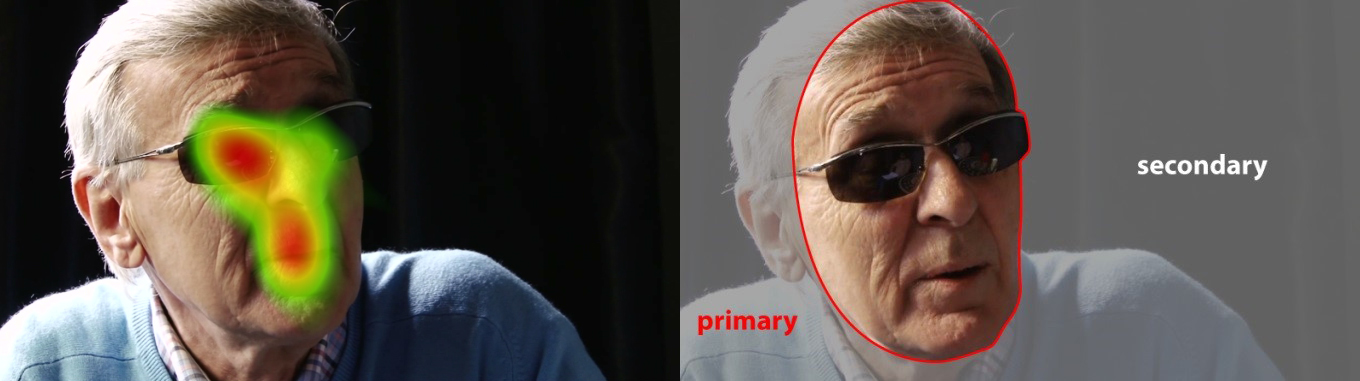
\includegraphics[width=\textwidth]{figures/FIG52fig49.jpg}
\caption{Fixation points of English natives (left) and resulting primary/secondary areas (\textit{Joining the Dots}, 00:00:48)}
\label{fig:FIG52fig49}
\end{figure}

Aside from these rather static image compositions, \textit{Joining the Dots} includes some more repetitive concepts. Images with mainly blurred or fast moving elements underline the interviewee’s statements, for example as Trevor speaks about the progressing loss of his sight (see \figref{fig:FIG53fig50}).

\begin{figure}
\includegraphics[width=\textwidth]{figures/FIG53fig50.jpg}
\caption{Scenes that support the overall atmosphere in \textit{Joining the Dots} (00:00:42, 00:01:20)}
\label{fig:FIG53fig50}
\end{figure}
 

The German subtitles were created according to the traditional guidelines described in \sectref{sec:1.2}. The integrated titles consisted of the same translation but were modified according to the discussions in the previous chapters.


  
\subsection{Adjustments to the conventional subtitles}\label{sec:7.5.3}

Adjustments were made regarding the conventional guidelines for subtitling, the \isi{placement} of the titles, and the \isi{layout} of the titles. These adjustments are presented in the following sections.

\subsubsection{Guidelines}\label{sec:7.5.3.1}

For the integrated titles for \textit{Joining the Dots}, the conventional guidelines presented in \sectref{sec:1.2} were modified. The ellipses (three dots) were omitted at the end respectively beginning of sentences connecting over multiple titles due to the clear sentence structures in the documentary and the audiovisual information channels. As the participants in this study form a hearing audience, the film provides sufficient information whether a sentence was completed yet or not. Instead, ellipses at the end of a title were used to indicate hesitation or an uncompleted sentence. Commas at the end of a title were left out as the pause between two consecutive titles in combination with the auditive information was deemed sufficient. As spoken content of different speakers is not displayed in the same title in integrated titles, dashes as indication of dialogue are omitted as well – the individual positions of the titles as well as the audiovisual information should allow an identification of the speakers. Depending on the \isi{image composition} and available contrast option, long one-liners and shorter two-line titles alternate. The shorter two-line titles, however, are usually more suitable due to their smaller horizontal space requirements. Furthermore, the need for italics to indicate “distant voices” (\citealt{Leisner2009}:~34, author’s translation; see also \sectref{sec:1.2}) was questioned, as image and plot allow an easy \isi{speaker identification} for the most part of the documentary. Therefore, no italics were used to indicate a speaker outside the frame. Even though this version of \textit{Joining the Dots} is intended for a hearing audience and the modifications are based on the assumption that the audience can connect the visible with the audible content, adjustments such as the individual \isi{placement} might already provide additional information for the hearing-impaired. For a more accessible translation, useful visual elements would have to be re-evaluated and adjusted to the requirements of the respective target group.

\subsubsection{Placement}\label{sec:7.5.3.2}

As the interviews are the main element of the documentary, it was decided not to place each title individually but to rather define consistent areas for the three interviewees. Therefore, Trevor’s titles are displayed in the right half of the image as he tends to look to the right. The titles for Joan Greening and Mags Silbery are displayed on the left half as they tend to look to the left. These positions were also supported by the positions of the captions with their names (see \figref{fig:FIG50fig47}) and the secondary areas in the corresponding shot compositions. For dialogues with two visible speakers in the image, the title positions would also indicate \isi{speaking direction}, if possible (see \figref{fig:FIG54fig51}). Overall, all titles were place as close as possible to the main \isi{focus point} in the respective scene to create small saccades between the fixations of title and image. Relevant image areas or elements were not to be covered by titles.

\begin{figure}
\includegraphics[width=\textwidth]{figures/FIG54fig51.png}
\caption{Indication of speaking direction in \textit{Joining the Dots} (00:06:01)}
\label{fig:FIG54fig51}
\end{figure}

\figref{fig:FIG55fig52} illustrates how the secondary areas usually allowed for a \isi{sufficient contrast}. Keeping the variety of title positions to a minimum, even if the \isi{shot composition} changes noticeably, might allow for more accessible adjustment, for instance for a hearing-impaired or \isi{deaf audience}. For such an audience, with a possibly greater need for additional visual information, speaker-related positions allow for faster identification of the speaker, even if he or she is not visible on the screen. Colour is another possibility to make identification easier, even though it is not always easy to come up with a suitable \isi{colour concept} for a film that works throughout the whole story.

\begin{figure}[t]
\includegraphics[width=\textwidth]{figures/FIG55fig52.jpg}
\caption{Roughly defined areas for Trevor (to the right of the speaker) and Mags (to the left of the speaker) in \textit{Joining the Dots} (00:00:54, 00:09:40)}
\label{fig:FIG55fig52}
\end{figure}

\subsubsection{Typography}\label{sec:7.5.3.3}

The original version of \textit{Joining the Dots} uses two typefaces: Today’s MS Office standard \isi{typeface} \textit{Calibri}\footnote{For further information on the \isi{typeface} \textit{Calibri}, see \url{http://www.lucasfonts.com/case-studies/calibri-consolas}/ [2014--12--29].} to display names (see \figref{fig:FIG50fig47}) and \textit{Slab Serif}\footnote{For further information on the \isi{typeface} \textit{Slab Serif}, see \url{http://www.linotype.com/3493/introduction.html} [2014--12--29].} for the \isi{film title}, creating a simple but noticeable tone (see \sectref{sec:2.3} on \isi{typographic film identity}). The closing credits are a mixture of both typefaces. The \isi{title design} for \textit{Joining the Dots} was based on a detailed interview with the director Pablo Romero-Fresco and the analysis of the existing examples of integrated titles and creative solutions (see \chapref{placement}). After various \isi{typographic} tests with typefaces and spatial effects, the \isi{typeface} \textit{Gill Sans} was chosen for the titles. The \isi{typeface} was not only chosen for its appearance but also for the graphic designer behind it: Eric Gill,\footnote{For further information on Eric Gill, see \url{http://www.ericgill.org.uk/Gill/} [2014--12--05].} an important English sculptor, typographer and graphic designer. The very British elements and characteristics of the documentary should also be visible in the \isi{typeface}, and as “Gill Sans [is] part of the British visual heritage just like the Union Jack and the safety pin” \citep{Archer2007}, it met this criterion. Besides the historic reference to the United Kingdom, \textit{Gill Sans Bold} is suitable as a screen \isi{typeface} due to its high \isi{legibility} – the bold style’s higher stroke weight ensures a good contrast and the clear design is unlikely to distract from the content. The \isi{film title} itself was not to be replaced during translation but rather to be accompanied by an additional title. To underline the individuality of the project but also the manual translation act – a little reminder of the fact that a translator was at work and, at least for this project, even part of the film production –, the handwritten \isi{typeface} \textit{Dakota}\footnote{For further information on the \isi{typeface} \textit{Dakota}, see \url{https://www.vletter.com/downloads/dakota-font-download-free.html} [014--12--17].} was chosen (see \figref{fig:FIG56fig53}).

\begin{figure}
\includegraphics[width=\textwidth]{figures/FIG56fig53.jpg}
\caption{The typefaces \textit{Dakota} (left) and \textit{Gill Sans Bold} (right) were chosen based on the analysis of the existing typographic identity of the film (\textit{Joining the Dots}, 00:00:10)}
\label{fig:FIG56fig53}
\end{figure}

In addition to these \isi{layout} decisions, a small number of effects were used to support the film’s atmosphere and tone. Slower fade in and fade outs were used to illustrate hesitation, unfinished sentences (slow fade out at the end), and sadness. If a speaker would move minimally through the \isi{title area}, a depth effect was used, meaning the speaker would partially cover the title (see \figref{fig:FIG57fig54}).

\begin{figure}
\includegraphics[width=\textwidth]{figures/FIG57fig54.png}
\caption{Depth effect after the title was displayed for a sufficiently long time (\textit{Joining the Dots}, 00:04:30)}
\label{fig:FIG57fig54}
\end{figure}

\largerpage
Finally, transparency was used to indicate the volume of speech (100\,\% transparency being normal volume and less transparency illustrating lower volume) or lessen a too strong contrast with the background of the title that would make the titles be more dominant than the rest of the image.

\section{Summary}\label{sec:7.6}

This chapter provided an overview over the pilot study, the resulting hypotheses, and the main study. This includes the experiment setup, participants, and used film material. Several adjustments were made to the traditional subtitles in order to create the set of integrated titles for \textit{Joining the Dots}. Using a Tobii TX300 \isi{eye tracker}, the eye movements of 45 participants were recorded watching the English short documentary \textit{Joining the Dots} in three conditions: original (unsubtitled), subtitled, and with integrated titles. Of these participants, 14 were English native participants watching the original and 31 were German participants dependent on translation watching the film with either traditional subtitles (15 participants) or integrated titles (16 participants). The integrated titles follow a distinct set of rules concerning \isi{layout} and \isi{placement}, and the 16 participants watching the film with integrated titles were asked to fill in a \isi{post-hoc questionnaire} on their \isi{information intake} and \isi{aesthetic experience}. The results of both the \isi{eye tracking} recordings and the questionnaire data are presented in the following chapter.

